\documentclass[11pt,a4paper]{article}

\usepackage[T1]{fontenc}
\usepackage[utf8]{inputenc}
\usepackage[margin=2.5cm]{geometry}
\usepackage{mathptmx}
\usepackage[scaled=0.9]{helvet}
\usepackage{courier}
\usepackage{microtype}
\usepackage{amsmath}
\usepackage{booktabs}
\usepackage{tabularx}
\usepackage{array}
\usepackage{caption}
\usepackage{pgfplots}
\pgfplotsset{compat=1.18}
\usepackage[round,authoryear]{natbib}
\usepackage{xcolor}
\usepackage[hidelinks]{hyperref}
\usepackage{url}
\usepackage{longtable}
\setlength{\LTpre}{6pt}\setlength{\LTpost}{8pt}

\usepackage{needspace}
\usepackage{etoolbox}
% Layout: never leave a heading stranded at the bottom of a page.
% A section needs room for its heading plus about 8 lines of text,
% a subsection about 6 lines; otherwise it starts on the next page.
\pretocmd{\section}{\needspace{10\baselineskip}}{}{}
\pretocmd{\subsection}{\needspace{7\baselineskip}}{}{}
% No single first/last lines of a paragraph alone on a page.
\clubpenalty=10000
\widowpenalty=10000
\displaywidowpenalty=10000
% Let pages end short instead of stretching the vertical space.
\raggedbottom
% Allow floats to take more of a page, so tables stay near their text.
\renewcommand{\topfraction}{0.85}
\renewcommand{\textfraction}{0.15}
\renewcommand{\floatpagefraction}{0.75}
\newcommand{\x}{\ensuremath{\times}}
\newcolumntype{L}{>{\raggedright\arraybackslash}X}
\definecolor{accent}{RGB}{38,110,210}
\definecolor{muted}{RGB}{190,190,180}

\title{The Byte Tax: Technical Report\\[4pt]\large Profiling Byte-Level Language Model Decoding on a Consumer GPU}
\author{Fabio-Eric Rempel\\[2pt]
  \small Independent researcher, Detmold, Germany\\
  \small ORCID \href{https://orcid.org/0009-0008-8447-6159}{0009-0008-8447-6159}}
\date{November 2026\\[2pt]\small Version 1.0.0 \quad \href{https://doi.org/10.5281/zenodo.23924377}{doi:10.5281/zenodo.23924377}}

\begin{document}
\maketitle
\tableofcontents
\bigskip
\section*{Summary}\addcontentsline{toc}{section}{Summary}

This report is the full record behind the paper \emph{The Byte Tax: Decode Speed of Byte-Level Language Models on a Consumer GPU}, published in the same Zenodo record (\href{https://doi.org/10.5281/zenodo.23924377}{doi:10.5281/zenodo.23924377}). It documents the 13 studies in the order they were run, all 67 pre-registered hypotheses with verdicts, the negative results and the corrections made along the way. The paper presents the argument; this report keeps every number it rests on.

Byte-level language models remove the tokenizer, but at batch size 1 they decode about 2.4\x{} slower per generated byte than the token model they were derived from. We profile Bolmo 1B, a byteified OLMo 2 1B, against its source on a consumer GPU (RTX 3060 Ti) through a sequence of pre-registered interventions. In eager Hugging Face decoding, launch and host overhead dominate both models; the byte model suffers more because its local encoder and decoder run once per byte. Capturing the decode step in CUDA graphs and replacing the host loop with a single-sync loop speeds Bolmo up 3.8\x{} (15.0 to 3.97 ms/byte), byte-identically, and shrinks the gap to 1.54\x{}. The remaining gap follows a memory-bandwidth model: Bolmo reads about 1.0 GB of weights per output byte, OLMo about 0.75 GB. Weight-only quantization confirms this model by intervention and shows that the per-byte local stack is the cheapest place to quantize: it saves 4.1\x{} more time per GB quantized than the global model, at lower quality cost. With both models at their best quantization, the byte tax stabilizes at 1.4 to 1.5\x{} across bf16, int8 and int4. Most of what remains is per-kernel overhead from 574 small kernels per byte. Speculative drafting within patches makes Bolmo another 15 to 18\% faster and stays exact in fp32, but it makes OLMo 2 1.89\x{} faster, so the byte tax grows from 1.49\x{} to 2.37\x{}: at batch 1, verifying several tokens is almost free for a token model, while a byte model can amortize only its local stack. Aligning drafting rounds to patch boundaries reverses this: Bolmo becomes 2.06\x{} faster than its minimal loop in bf16, and the drafted byte tax falls to 1.36\x{}, below the undrafted 1.49\x{}. Skinny matmul kernels then make int8 global weights near-lossless at 1.59 ms/byte, but widen the tax to 1.60\x{}, because the token model's time is more dominated by weight reads. Twenty-six of 67 pre-registered hypotheses were refuted and five partly, including our own predictions that the host loop dominated and that drafting would leave the byte tax unchanged; all are reported.

\section{Introduction}\label{introduction}

Byte-level models are promising on quality but are rarely used, partly because decoding them is assumed to be slow. Recent work closes the quality gap cheaply: byteification retrofits an existing subword model to bytes with under 1\% of a pretraining budget \citep{minixhofer2026byteification}. Whether the speed gap is fundamental or an artifact of unoptimized inference has not been measured on consumer hardware.

Research questions:

\begin{enumerate}
\def\labelenumi{\arabic{enumi}.}
\item
  Where does decode time go in a byteified model, compared with its token-level source, under identical conditions?
\item
  How much of the gap is overhead (launches, host syncs) that standard techniques remove?
\item
  Does the remaining gap follow a memory-bandwidth model, and which part of the byte model carries it?
\item
  Is that part unusually cheap to quantize, in speed and in quality?
\item
  What is left after all of the above, and what would remove it?
\end{enumerate}

Contributions: a reusable profiling harness; a chain of pre-registered interventions on Bolmo 1B and OLMo 2 1B; a bandwidth model validated by quantization; the finding that the per-byte local stack is the most efficient quantization target; and a decomposition of the remaining per-kernel floor.

\section{Setup}\label{setup}

All main results come from one RTX 3060 Ti (8 GB) under Windows, bf16, batch size 1, greedy decoding, fixed seed, and a fixed five-prompt set (English, Python, German, JSON, mixed Unicode). A Colab Tesla T4 (Linux, fp32) serves as a cross-check.

\begin{center}\small\setlength{\tabcolsep}{4pt}
\begin{tabular}{@{}>{\raggedright\arraybackslash}p{\dimexpr 0.204\linewidth-2\tabcolsep\relax}>{\raggedright\arraybackslash}p{\dimexpr 0.796\linewidth-2\tabcolsep\relax}@{}}
\toprule
\textbf{Item} & \textbf{Detail} \\
\midrule
Byte model & Bolmo 1B \citep{minixhofer2026byteification} (allenai/Bolmo-1B, pinned revision 452690a8): 1 mLSTM encoder layer, 16 global transformer layers, 4 mLSTM decoder layers, fused 512+8 output vocabulary \\
Token model & OLMo 2 1B \citep{walsh2025olmo2} (allenai/OLMo-2-0425-1B), the source Bolmo 1B was byteified from \\
Output length & 256 new bytes; OLMo set to 72 tokens (about 259 bytes) so KV-cache sizes match \\
Metric & ms per generated UTF-8 byte; no-hook wall time for headline numbers \\
Quality & bits per byte on the first 200,000 bytes of WikiText-2 test; CUTE \citep{edman2024cute} accuracy on 1,500 seeded items (500-item subset kept for comparability) \\
Software & transformers 4.57.3, torch, triton-windows, xlstm 2.0.6, mlstm\_kernels 2.0.6, torchao 0.9.0 (exact versions in requirements.txt) \\
\bottomrule
\end{tabular}
\end{center}

Harness (byteprof): forward hooks with CUDA events give per-component times; a no-hook run of the same workload gives true throughput and hook overhead (5 to 7\%). Optimized variants run without hooks, because graph replay bypasses them. Traces come from torch.profiler on Linux and Nsight Systems on Windows.

Protocol: each step was a written task with hypotheses copied verbatim into FINDINGS.md before any measurement and never edited afterwards. Two runs per variant; any pair differing by more than 5\% was rerun and the outlier reported. Optimized outputs were compared byte for byte with eager output.

\section{Results}\label{results}

Bolmo's decode cost falls from 15.0 to 1.99 ms per byte (7.5\x{}) through five interventions; the ratio to an equally optimized OLMo 2 settles at 1.4 to 1.5\x{}. Drafting aligned to patch boundaries then takes it to 1.46 ms/byte in int4 (10.3\x{}) and 1.93 in bf16, and narrows the ratio to 1.36\x{} (section 3.12). Figure\textasciitilde \ref{fig:cascade} shows the cascade.

\begin{figure}[tb]
\centering
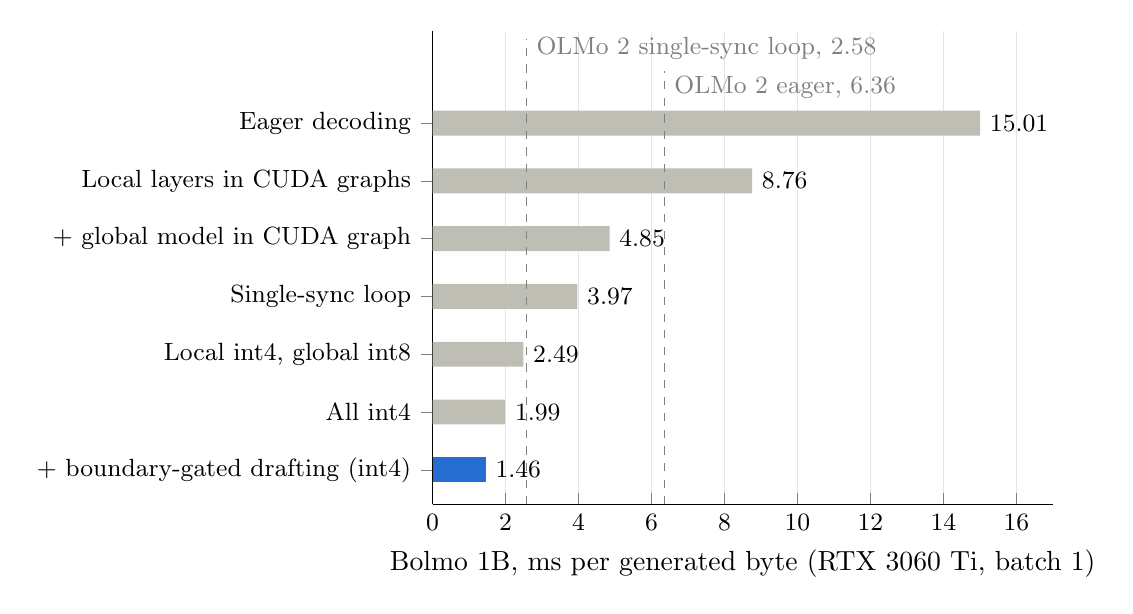
\begin{tikzpicture}
\begin{axis}[
  xbar,
  bar shift=0pt,
  width=0.78\textwidth,
  height=7.6cm,
  bar width=9pt,
  xmin=0, xmax=17,
  ymin=0.4, ymax=8.6,
  xlabel={Bolmo 1B, ms per generated byte (RTX 3060 Ti, batch 1)},
  ytick={1,2,3,4,5,6,7},
  yticklabels={
    {+ boundary-gated drafting (int4)},
    {All int4},
    {Local int4, global int8},
    {Single-sync loop},
    {+ global model in CUDA graph},
    {Local layers in CUDA graphs},
    {Eager decoding}},
  y tick label style={font=\small},
  x tick label style={font=\small},
  nodes near coords,
  nodes near coords style={font=\small},
  point meta=x,
  every node near coord/.append style={/pgf/number format/fixed,/pgf/number format/fixed zerofill,/pgf/number format/precision=2},
  axis x line*=bottom,
  axis y line*=left,
  xmajorgrids=true,
  grid style={gray!20},
  clip=false,
]
\addplot[fill=muted, draw=none] coordinates {
  (15.01,7) (8.76,6) (4.85,5) (3.97,4) (2.49,3) (1.99,2)};
\addplot[fill=accent, draw=none] coordinates {(1.456,1)};
\draw[dashed, gray] (axis cs:6.36,0.4) -- (axis cs:6.36,7.9);
\node[anchor=west, font=\small, text=gray] at (axis cs:6.36,7.62) {OLMo~2 eager, 6.36};
\draw[dashed, gray] (axis cs:2.58,0.4) -- (axis cs:2.58,8.45);
\node[anchor=west, font=\small, text=gray] at (axis cs:2.58,8.3) {OLMo~2 single-sync loop, 2.58};
\end{axis}
\end{tikzpicture}
\caption{Bolmo's decode cost through the main interventions, each measured in its own study (bf16 unless noted; bf16 baselines agree within 0.5\% across sessions). Overhead removal (top four bars) gives 3.8\x, quantization 2.0\x{} and boundary-gated drafting a further 1.37\x. Dashed lines: OLMo~2~1B eager and with the same single-sync loop, bf16.}
\label{fig:cascade}
\end{figure}


Overhead removal (the first three steps) accounts for 3.8\x{}, quantization for 2.0\x{} and boundary-gated drafting for 1.37\x{}. Without quantization, gated drafting brings bf16 Bolmo to 1.93 ms/byte, 1.36\x{} drafted OLMo 2 in bf16 (1.42).

\subsection{Eager baseline}\label{eager-baseline}

In eager decoding Bolmo needs 15.0 ms per byte and OLMo 2 needs 6.36 (2.36\x{}). The global transformer costs about the same per byte in both (about 6.8 vs 6.4 ms), because a 3.38-byte patch compresses nearly as well as a 3.6-byte token. The whole gap is Bolmo's local encoder and decoder: about 9.0 ms per byte against 0.7 ms for OLMo's embedding, norm and head. A global layer costs about 1.4 ms per call in both models, roughly 4.4\x{} the bandwidth floor. On a Linux T4 (fp32) the GPU was busy only 35.5\% of the time for Bolmo and 63.8\% for OLMo, with about 430 and 220 kernels per byte; the ratio there was 2.09\x{}.

\subsection{Measurement correction}\label{measurement-correction}

A suspected harness bug (prompt counted as output) was refuted before any code changed. The real cause was in Bolmo's remote \texttt{generate()}: its length cap allows input length + max\_new - 3 new bytes, so the first runs were about 2.4\x{} too long. The harness now enforces the cap itself. On the T4, fp16 made Bolmo emit only special token 0 (overflow); the \texttt{inspect} check caught it, and Colab runs use fp32.

\subsection{Overhead removal (H1 to H4)}\label{overhead-removal-h1-to-h4}

Capturing Bolmo's five local layers in CUDA graphs cut its time by 41.6\% (15.01 to 8.76 ms/byte); adding the global model reached 4.85 ms/byte, 3.09\x{} faster than eager and byte-identical to it. \texttt{torch.compile} gave similar speed but diverged from eager output on two of five prompts. Against compiled OLMo (3.19 ms/byte) the ratio was 1.52\x{}, just above the pre-registered 1.5\x{} line (H3 refuted).

\subsection{Minimal-sync loop (H5 to H10)}\label{minimal-sync-loop-h5-to-h10}

Bolmo's host loop made 9 syncs per byte but cost only 1.0 ms of the 4.85 (21\%, H5 refuted). The O(n) history walk for subword ids cost 47 microseconds per call and did not grow measurably with length (H6 refuted). A single-sync loop with an Aho-Corasick automaton for subword ids, exact against the tokenizer on about 30,000 positions, brought Bolmo to 3.97 ms/byte. Given the same loop, OLMo reached 2.58, so the gap stayed at 1.54\x{} (H7 to H9 refuted).

\subsection{Bandwidth model, tested by quantization (H11 to H16)}\label{bandwidth-model-tested-by-quantization-h11-to-h16}

Bolmo reads about 1.0 GB of weights per output byte (0.64 GB global, 0.36 GB local), OLMo about 0.75 GB. Weight-only quantization of either part produced savings at a steady 71 to 77\% of the bandwidth model's prediction. A fit of time = fixed + k x weight bytes matches all variants within about 2\% and puts the fixed part near 1.15 ms/byte. Per GB quantized, local weights save 4.06\x{} more time than global weights (H14), close to the 3.4\x{} expected from being read once per byte instead of once per patch.

\subsection{Fair ratio, global int8, floor (H17 to H20)}\label{fair-ratio-global-int8-floor-h17-to-h20}

With matched kernels and loops, each model at its best precision gives a ratio of 1.49\x{} (bf16), 1.40\x{} (int8) and 1.48\x{} (int4). Keeping both output heads in bf16 gives 1.12\x{} at int4, because OLMo's 421 MB head costs 0.43 ms/byte and Bolmo's head is tiny. At all-int4, Bolmo's 2.0 ms/byte splits into matmuls 0.80, other kernels 0.98, in-graph gaps 0.12 and host work 0.10. It runs 574 kernels per byte, 547 of them under 10 microseconds, at about 1 microsecond minimum per graph node. Syncs (0.03 to 0.05 ms) and mLSTM state traffic (0.05 to 0.07 ms) are negligible.

\subsection{Speculative drafting (H21 to H28)}\label{speculative-drafting-h21-to-h28}

Within-patch speculative drafting \citep{leviathan2023speculative,chen2023speculative} makes Bolmo 15 to 18\% faster, but the same treatment makes OLMo 2 1.89\x{} faster, so the byte tax grows from 1.49\x{} to 2.37\x{}.

Drafter: context lookup first \citep{saxena2023promptlookup}, then a byte n-gram model built from a 19.4 MB corpus (WikiText-2 train, Python standard library, German book text), with no 32-byte window shared with any prompt. Parameters were tuned on 25 extended prompts, not on the 5 used for timing. It emits 2.0 to 2.3 bytes per local pass at 256 new bytes, against 3.7 for an oracle. Repetition flatters it: half of all 8-byte windows in the outputs occur earlier in prompt or output.

Verification: the encoder and decoder run over K+1 positions in one CUDA graph. Projections and MLPs are batched over the rows; the mLSTM recurrence runs as K+1 sequential steps that keep the state after every position, so rollback is an index. Acceptance runs on the GPU, and the host syncs once per round. A round with K = 4 costs 1.245\x{} a single step in bf16 and 1.320\x{} in int4. The cost model predicted the measured gains within 7\%.

Same-session comparison, bf16, default prompts, 256 new bytes:

\begin{center}\small\setlength{\tabcolsep}{4pt}
\begin{tabular}{@{}>{\raggedright\arraybackslash}p{\dimexpr 0.363\linewidth-2\tabcolsep\relax}>{\raggedright\arraybackslash}p{\dimexpr 0.256\linewidth-2\tabcolsep\relax}>{\raggedright\arraybackslash}p{\dimexpr 0.211\linewidth-2\tabcolsep\relax}>{\raggedright\arraybackslash}p{\dimexpr 0.170\linewidth-2\tabcolsep\relax}@{}}
\toprule
\textbf{Model} & \textbf{Minimal loop (ms/byte)} & \textbf{Drafted (ms/byte)} & \textbf{Speedup} \\
\midrule
Bolmo 1B (combined drafter, K = 6) & 3.995 & 3.361 & 1.19\x{} \\
OLMo 2 1B (combined drafter, K = 8) & 2.688 & 1.420 & 1.89\x{} \\
Ratio Bolmo / OLMo 2 & 1.49\x{} & 2.37\x{} &  \\
\bottomrule
\end{tabular}
\end{center}

In all-int4, drafting takes Bolmo from 1.994 to 1.703 ms/byte (1.17\x{}).

Why the asymmetry: at batch 1, a pass reads all weights once whether it processes one position or nine, and the GPU's compute is mostly idle, so OLMo verifies 9 tokens for 8\% more than 1. Bolmo can batch only its local stack, about 37 to 40\% of its time; the global model still runs once per patch. Its mLSTM recurrence must step through drafted positions in sequence, and each round stops at the next patch boundary.

Exactness: in fp32 the drafted output equals the non-drafted output in every run (Bolmo 240 of 240 over four drafters, OLMo 60 of 60, plus a CPU toy-model test that catches four injected rollback bugs). In bf16 and int4, 30\% of runs diverge, always at a near-tie of the top two logits (gap at most 0.125), where a batched matmul rounds differently from a single row. On the 3 default prompts with identical bf16 output, the speedup is 1.116\x{}.

Multi-patch drafting would also batch the global model, which costs only 1.07\x{} for four patches in one pass. The cost model still predicts at most 4.9\% over within-patch drafting in bf16 and a 6 to 10\% loss in int4, because the global model would then run in almost every round. It was not built.

\subsection{Cheaper local verification (H29 to H33)}\label{cheaper-local-verification-h29-to-h33}

A fused multi-step mLSTM kernel made the recurrence cheap but sped up drafted decoding by only about 1\%, because the real cost of verifying several bytes sits in the small matrix multiplications.

\begin{itemize}
\item
  The kernel loops over all drafted positions with the state on chip and, after acceptance, recomputes the state only up to the accepted position. The recurrence fell from 16.1 to 4.5 microseconds per extra position across the five layers. fp32 output stayed identical in 60 of 60 runs.
\item
  End to end: 3.330 vs 3.352 ms/byte in bf16 (+0.7\%), 1.691 vs 1.715 in int4 (+1.4\%). The cost model predicted +1.2\% and +1.5\%; the 5 to 8\% predicted beforehand rested on a wrong state size (512 KiB per layer, not 1 MiB).
\item
  Where the cost goes instead: for one row cuBLAS uses gemv kernels tuned for decoding; for two or more rows it switches to gemm kernels with 64x64 tiles, mostly padding at 2 to 9 rows. One small gate projection goes from 3.5 to 10.8 microseconds. int4 tinygemm adds 28 to 45 microseconds per extra row.
\item
  For crossing drafts: in bf16 a K = 16 round costs only +0.48 ms against a 7.7 ms global pass, so large K is affordable; in int4 a K = 16 round costs 2.09\x{} a single step.
\end{itemize}

A skinny-matrix kernel for 2 to 16 rows, reading each weight once for all rows, is the remaining lever here. Its ceiling is about 5.7\% in bf16 and 7.4\% in int4.

\subsection{Drafts that cross patch boundaries (H34 to H38)}\label{drafts-that-cross-patch-boundaries-h34-to-h38}

Crossing patch boundaries pays as soon as a round emits about one patch of bytes, but no available drafter is both accurate and cheap enough, so it was not built.

\begin{itemize}
\item
  Boundary flags are predictable: Bolmo's flags match the OLMo 2 tokenizer's splits of its own output on 98.7\% of byte positions and 95.0\% of patches. German is the exception (80.6\% of patches), where Bolmo keeps compounds such as Eisenbahn together.
\item
  Break-even: one global pass over 1 to 8 patches costs 7.69 to 8.33 ms in bf16, almost flat, so crossing beats within-patch drafting from about 1.01 to 1.07\x{} the bytes per patch, not the 1.2\x{} predicted.
\item
  Accuracy: the best of three small token models (SmolLM2-135M, SmolLM2-360M, Qwen2.5-0.5B) emits 4.52 bytes per round at K = 32; only about 25\% of rounds cross a boundary. One wrong token ends a round, and a 135 to 500M model predicts the exact next word of the 1B target about one time in two.
\item
  Cost: one draft token costs 3.7 to 5.5 ms against a whole Bolmo round of 1.4 to 2.0 ms. Even at the drafter's weight-bandwidth floor the best cell is 33.5\% slower than within-patch drafting; a free drafter would give +22\% in bf16 and nothing in int4.
\item
  The existing lookup drafter crossing patches is predicted at +6.1\% in bf16, below the 10\% gate. With OLMo 2 using the same small drafters, the model predicts the byte tax would rise to about 3.0\x{} (2.89\x{} after correct token healing; an earlier figure of 3.5\x{} mixed two prompt sets).
\end{itemize}

\subsection{Why drafting favors coarse units (H39 to H41)}\label{why-drafting-favors-coarse-units-h39-to-h41}

The same drafter continuations give OLMo 2 about 2.7\x{} the bytes per round that Bolmo gets, and the cause is the round protocol, not the text or the drafter's accuracy.

\begin{center}\small\setlength{\tabcolsep}{4pt}
\begin{tabular}{@{}>{\raggedright\arraybackslash}p{\dimexpr 0.542\linewidth-2\tabcolsep\relax}>{\raggedright\arraybackslash}p{\dimexpr 0.458\linewidth-2\tabcolsep\relax}@{}}
\toprule
\textbf{Factor (SmolLM2-360M drafter)} & \textbf{Effect on bytes per round, OLMo vs Bolmo} \\
\midrule
Text (OLMo's output is slightly harder to predict) & 0.89\x{} \\
Boundary flags must match (Bolmo only) & 1.05\x{} \\
Free unit per round and restart position & 2.6\x{} \\
Byte vs token matching & 1.1\x{} \\
Total & 2.65\x{} \\
\bottomrule
\end{tabular}
\end{center}

\begin{itemize}
\item
  Per-token agreement is about equal for both models (72 to 80\%), so the drafter is not better at predicting OLMo.
\item
  Free unit: every round ends with one unit the target predicts itself, a token (about 4 bytes) for OLMo, one byte for Bolmo.
\item
  Restart position: 68\% of Bolmo's rounds restart inside a token, where a token-level drafter is right 25 to 30\% of the time (67 to 73\% after correct token healing), against 86 to 94\% at a token boundary. Mid-token rounds emit 1.8 bytes; rounds starting at a token end emit 9.8.
\item
  This is tokenization bias \citep{phan2025exact} appearing inside speculative decoding: a token model conditioned on a context that ends mid-token predicts poorly, and byte-level verification keeps handing the drafter such contexts.
\item
  Correct healing raised Bolmo's best cell only from 4.52 to 4.62 bytes per round, so the crossing-drafts verdict stands.
\end{itemize}

Byte models do not make more hard guesses than token models; by the chain rule, a span has the same probability however it is cut, and the uncertainty sits at word and patch starts. They make more steps, and drafting rounds end at byte granularity. Granularity is only part of why mid-token rounds are short: a round restarts right where the drafter just missed, and there its first byte is right only 17 to 23\% of the time, against 77 to 86\% elsewhere. The one-byte free unit and the short rest of the token explain 21 to 32\% of the shortfall; the rest is a selection effect, because misses cluster at hard positions, which in a byte model fall mid-token.

\subsection{Patch-aligned rounds (H42 to H47, simulation and cost model)}\label{patch-aligned-rounds-h42-to-h47-simulation-and-cost-model}

Gating crossing drafts to rounds that start at a patch boundary is predicted to make drafted Bolmo 33\% faster in bf16 (2.259 vs 3.377 ms/byte), and would bring the drafted byte tax from 2.38\x{} back to about 1.6\x{}.

\begin{center}\small\setlength{\tabcolsep}{4pt}
\begin{tabular}{@{}>{\raggedright\arraybackslash}p{\dimexpr 0.281\linewidth-2\tabcolsep\relax}>{\raggedright\arraybackslash}p{\dimexpr 0.184\linewidth-2\tabcolsep\relax}>{\raggedright\arraybackslash}p{\dimexpr 0.216\linewidth-2\tabcolsep\relax}>{\raggedright\arraybackslash}p{\dimexpr 0.184\linewidth-2\tabcolsep\relax}>{\raggedright\arraybackslash}p{\dimexpr 0.136\linewidth-2\tabcolsep\relax}@{}}
\toprule
\textbf{bf16, default prompts} & \textbf{Expensive passes per byte} & \textbf{Approx. cost of those (ms/byte)} & \textbf{Everything else (ms/byte)} & \textbf{Total (ms/byte)} \\
\midrule
Bolmo, within-patch lookup drafting (P0) & 0.263 global & 2.0 & 1.35 & 3.38 \\
Bolmo, boundary-gated lookup (P4, predicted) & 0.139 global & 1.1 & 1.15 & 2.26 \\
OLMo 2, lookup drafting & 0.130 full model & 1.3 & 0.1 & 1.42 \\
\bottomrule
\end{tabular}
\end{center}

The split into pass cost and remainder is derived from passes per byte and measured pass costs and is approximate.

\begin{itemize}
\item
  Policy: mid-patch rounds keep cheap within-patch lookup drafting; a round that starts at a boundary drafts across patches with the lookup drafter and flags from tokenizer re-segmentation, and one global pass covers several patches. Bytes per global pass rise from 3.8 to 7.2.
\item
  With P4, Bolmo makes about as few expensive passes per byte as drafted OLMo 2. What remains of the byte tax is the local stack, about 1.1 ms per byte.
\item
  Crossing every round (P1) gains only 5\%, because it pays a global pass in every round. P4 beats P1 by 29\%, which the pre-registered prediction (a few percent) missed.
\item
  LM drafters: a hybrid draft (lookup completion of the patch, then the LM) reaches 5.6 bytes per round; gating the LM to boundary rounds ties P4 only if the drafter ran at its bandwidth floor, and is 45\% slower than P0 at measured cost. Lookup completion accuracy, not the LM, limits the hybrid.
\item
  int4: P4 is +24\% on the extended prompts but only +8.9\% on the default prompts.
\item
  A two-state model (rounds restart at a boundary or mid-patch) reproduces simulated bytes per round within 1.3\% in-sample, which is close to an identity; on held-out prompts 3 of 16 cells miss by more than 10\%.
\item
  Not yet measured: the cost of a multi-patch decoder and pooling several patches. The bf16 gain survives up to about +2 ms per crossing round (+24\%).
\end{itemize}

\subsection{Boundary-gated drafting, built (H48 to H53)}\label{boundary-gated-drafting-built-h48-to-h53}

Built and measured, boundary-gated drafting makes Bolmo 2.06\x{} faster than its minimal loop in bf16 and narrows the drafted byte tax to 1.36\x{}, below the undrafted 1.49\x{}.

\begin{center}\small\setlength{\tabcolsep}{4pt}
\begin{tabular}{@{}>{\raggedright\arraybackslash}p{\dimexpr 0.505\linewidth-2\tabcolsep\relax}>{\raggedright\arraybackslash}p{\dimexpr 0.495\linewidth-2\tabcolsep\relax}@{}}
\toprule
\textbf{bf16, same session} & \textbf{Bolmo / OLMo 2 ratio} \\
\midrule
Neither model drafts & 1.48\x{} \\
Both draft, Bolmo within patches only & 1.97\x{} (2.37\x{} in the earlier session) \\
Both draft, Bolmo boundary-gated & 1.36\x{} \\
\bottomrule
\end{tabular}
\end{center}

Default prompts, 256 new bytes, two runs per cell (pair gaps at most 0.8\%):

\begin{center}\small\setlength{\tabcolsep}{4pt}
\begin{tabular}{@{}>{\raggedright\arraybackslash}p{\dimexpr 0.155\linewidth-2\tabcolsep\relax}>{\raggedright\arraybackslash}p{\dimexpr 0.140\linewidth-2\tabcolsep\relax}>{\raggedright\arraybackslash}p{\dimexpr 0.239\linewidth-2\tabcolsep\relax}>{\raggedright\arraybackslash}p{\dimexpr 0.249\linewidth-2\tabcolsep\relax}>{\raggedright\arraybackslash}p{\dimexpr 0.218\linewidth-2\tabcolsep\relax}@{}}
\toprule
\textbf{ms/byte} & \textbf{Minimal loop} & \textbf{Best within-patch drafting} & \textbf{Boundary-gated} & \textbf{Gain vs within-patch} \\
\midrule
bf16 & 3.975 & 2.798 (K = 8) & 1.934 & +30.9\% \\
all-int4 & 1.998 & 1.686 (K = 4) & 1.456 & +13.6\% \\
\bottomrule
\end{tabular}
\end{center}

\begin{itemize}
\item
  A crossing round costs at most 0.10 ms (bf16) and 0.04 ms (int4) beyond the pieces already in the cost model, a tenth of the 1.0 ms allowed.
\item
  The real loop matches the simulation: 7.15 bytes per global pass on the extended set, exactly as simulated, about twice within-patch drafting.
\item
  Text confound: in bf16, near-tie divergences change the text of 3 of 5 default prompts, and the drafted text is more draftable. On the prompts whose text equals the minimal loop's, the gain over within-patch drafting is +37.9\% (bf16) and +15.1\% (int4). This also explains why the cost model was 12.6\% pessimistic in bf16 and exact in int4 (-0.1\%).
\item
  Exactness: fp32 output identical in bytes and flags for all 30 prompts at 256 and 1024 bytes; all 22 bf16 and int4 divergences sit at near-ties (top-2 logit gap at most 0.0625).
\item
  Time per byte in bf16: about 1.1 ms in global passes (0.135 per byte, about 8 ms each, flat in the number of patches), 0.6 ms in local rounds, 0.2 ms prefill and host. The global model is again 55 to 60\% of the time.
\end{itemize}

All six hypotheses were supported. H48 and H53 had loose thresholds; H49 (gain of at least 25\%) and H50 (cost model within 15\%) were the real tests, and the cost model had been calibrated by the earlier refutations.

\subsection{Skinny matmul kernels (H54 to H59)}\label{skinny-matmul-kernels-h54-to-h59}

A kernel family that reads each weight once for 1 to 64 rows makes int8 global weights usable in drafting rounds: Bolmo reaches 1.588 ms/byte at +0.002\% bits per byte, but the byte tax widens to 1.60\x{} because OLMo 2 gains more.

\begin{itemize}
\item
  Kernels (Triton, bf16, int8 and int4 weights, fp32 accumulation): int8 reaches 77 to 91\% of the measured 411 GB/s copy bandwidth at one row, and 8 rows cost 0.97 to 1.05\x{} one row. bf16 at 2 to 9 rows costs 0.81 to 0.99\x{} cuBLAS's single-row kernel, which removes the padded-tile penalty of section 3.8.
\item
  Near-lossless variant (int8 global, bf16 local): 1.588 vs 1.936 ms/byte for bf16 boundary-gated drafting, +17.9\%, short of the pre-registered 20\%. int8 flips a few near-tie bytes and the resulting text is less draftable (7.4 to 6.6 bytes per global pass); on identical text the gain is 25.0\%, against 25.7\% predicted.
\item
  The custom int4 kernel is 1.7\x{} slower than tinygemm at up to 4 rows, limited by dequantization arithmetic, and wins only from about 9 to 16 rows; all-int4 drafting with it is 11.7\% slower.
\item
  fp32 drafted output stays identical to non-drafted output for both models; kernel error at most 6.5e-4 against an fp32 reference.
\end{itemize}

\begin{center}\small\setlength{\tabcolsep}{4pt}
\begin{tabular}{@{}>{\raggedright\arraybackslash}p{\dimexpr 0.314\linewidth-2\tabcolsep\relax}>{\raggedright\arraybackslash}p{\dimexpr 0.321\linewidth-2\tabcolsep\relax}>{\raggedright\arraybackslash}p{\dimexpr 0.364\linewidth-2\tabcolsep\relax}@{}}
\toprule
\textbf{Optimization} & \textbf{Gains more} & \textbf{Why} \\
\midrule
Drafting within patches & OLMo 2 (1.89\x{} vs 1.19\x{}) & verification amortizes its whole model \\
int8 weights with skinny kernels & OLMo 2 (+26 to 30\% vs +18 to 23\%) & almost all its time is weight streaming \\
Patch-aligned drafting & Bolmo & it removes a cost only byte models have \\
\bottomrule
\end{tabular}
\end{center}

This is Amdahl's law: optimizations of weight reads help most the model whose time is mostly weight reads. With both models at int8 and drafting, Bolmo needs about 0.6 ms more per byte than OLMo 2, roughly the cost of its per-byte local stack. A global pass still spends about 2 of its 5 ms outside matmuls (attention, norms, rotary, cache writes), but fusing that would help OLMo 2's identical transformer equally and widen the ratio further.

\subsection{Megakernel theory, tested (H60 to H64)}\label{megakernel-theory-tested-h60-to-h64}

A persistent megakernel for the local step would not pay on this card: the overhead is kernel count, not synchronization or idle waiting, and at int8 the byte tax already sits only about 13\% above its hardware floor.

\begin{center}\small\setlength{\tabcolsep}{4pt}
\begin{tabular}{@{}>{\raggedright\arraybackslash}p{\dimexpr 0.615\linewidth-2\tabcolsep\relax}>{\raggedright\arraybackslash}p{\dimexpr 0.385\linewidth-2\tabcolsep\relax}@{}}
\toprule
\textbf{Mechanism} & \textbf{Measured on the RTX 3060 Ti} \\
\midrule
Kernel launches from the CPU & already removed by CUDA graphs \\
Barrier between phases (all blocks wait) & about 1 microsecond per phase \\
Dataflow waits (each block waits only for its producers) & saves 3 to 9\% of that \\
Prefetching the next phase's weights while waiting & -1 to +2 points of bandwidth \\
Persistent kernel vs the same 28 phases as a CUDA graph & 1123 vs 1126 microseconds \\
\bottomrule
\end{tabular}
\end{center}

\begin{itemize}
\item
  A bf16 local round takes 1385 microseconds against an 877 microsecond weight-read floor. Its 42 matmul kernels run within 4\% of the floor; the excess is 238 small non-matmul kernels (371 microseconds: norms, gate math, residuals, mLSTM glue) and 74 microseconds of gaps.
\item
  Prefetch does not help because the per-phase stall (5 to 8 microseconds) is the arrival of the slowest block's result, not weight loading, and one phase's weights (several MB) are far larger than a processor's on-chip memory.
\item
  The published megakernel gains \citep{hazy2025megakernel,cheng2026mpk} were measured against serving engines without this degree of graph capture; against a fused CUDA graph, little remains.
\item
  Predicted gain of a real local megakernel on top of boundary-gated drafting: +4.3\% (bf16 local) and +7.5\% (int4 local), below the 10\% gate. Fusing the small kernels would save about 0.2 ms per round, roughly 4 to 5\% end to end.
\end{itemize}

Bandwidth-floor ratio, both models at the floor with drafting, from real parameter counts and measured passes and rounds per byte:

\begin{center}\small\setlength{\tabcolsep}{4pt}
\begin{tabular}{@{}>{\raggedright\arraybackslash}p{\dimexpr 0.239\linewidth-2\tabcolsep\relax}>{\raggedright\arraybackslash}p{\dimexpr 0.426\linewidth-2\tabcolsep\relax}>{\raggedright\arraybackslash}p{\dimexpr 0.334\linewidth-2\tabcolsep\relax}@{}}
\toprule
\textbf{Precision} & \textbf{Floor ratio, local at same precision} & \textbf{Floor ratio, local in int4} \\
\midrule
bf16 & 1.23\x{} & 0.97\x{} \\
int8 & 1.42\x{} & 1.24\x{} \\
\bottomrule
\end{tabular}
\end{center}

The measured int8 ratio of 1.60\x{} is about 13\% above its floor; a perfect local megakernel would reach roughly 1.48 to 1.53\x{}. What lowers the floor itself is fewer local weight bytes per round (an int4 local stack) or more bytes per round (better drafts).

\subsection{Final frontier (H65 to H67)}\label{final-frontier-h65-to-h67}

Neither remaining configuration was predicted to clear the 8\% gate, so the optimization work ends here: Bolmo's byte tax on this card settles at about 1.4 to 1.6\x{} OLMo 2 at the same precision, 11 to 16\% above the bandwidth floor.

\begin{center}\small\setlength{\tabcolsep}{4pt}
\begin{tabular}{@{}>{\raggedright\arraybackslash}p{\dimexpr 0.305\linewidth-2\tabcolsep\relax}>{\raggedright\arraybackslash}p{\dimexpr 0.097\linewidth-2\tabcolsep\relax}>{\raggedright\arraybackslash}p{\dimexpr 0.097\linewidth-2\tabcolsep\relax}>{\raggedright\arraybackslash}p{\dimexpr 0.120\linewidth-2\tabcolsep\relax}>{\raggedright\arraybackslash}p{\dimexpr 0.188\linewidth-2\tabcolsep\relax}>{\raggedright\arraybackslash}p{\dimexpr 0.107\linewidth-2\tabcolsep\relax}>{\raggedright\arraybackslash}p{\dimexpr 0.086\linewidth-2\tabcolsep\relax}@{}}
\toprule
\textbf{Configuration (boundary-gated drafting)} & \textbf{ms/byte} & \textbf{bpb change} & \textbf{CUTE change (pts)} & \textbf{Ratio to OLMo 2, same precision} & \textbf{Floor ratio} & \textbf{Above floor} \\
\midrule
bf16, cuBLAS & 1.936 & 0 & 0 & 1.36\x{} & 1.23\x{} & +11\% \\
Global int8 + bf16 local, skinny (near-lossless) & 1.588 & +0.002\% & -0.13 & 1.60\x{} & 1.42\x{} & +13\% \\
Global int8 + local int4, skinny & 1.430 & +1.13\% & about -2.4 & 1.44\x{} (cross-session) & 1.24\x{} & +16\% \\
All int4, tinygemm & 1.462 & +4.9\% & -6.2 & not measured & not computed & \begin{itemize}
\item
\end{itemize} \\
A, predicted: local int8 + global int8 & 1.491 & about +0.08\% & about +0.2 & 1.50\x{} & 1.42\x{} & +5\% \\
B, predicted: local int4 (row-count dispatch) + global int8 & 1.477 & about +1.2\% & about -2.4 & 1.49\x{} & 1.24\x{} & +20\% \\
\bottomrule
\end{tabular}
\end{center}

\begin{itemize}
\item
  Predicted gains over the near-lossless cell: A +6.1\%, B +7.0\%, both under the 8\% gate. The local linears are only part of a local round, and the global pass, about half the time, is untouched.
\item
  The int4 kernel's per-row cost decides B: tinygemm alone gains 4.2\%; switching to the skinny kernel above about 8 to 12 rows adds about 2.8 points.
\item
  Caveat: the measured global-int8 + local-int4 cell runs 9.9\% faster than the reference because its generated text drafts better, which the model cannot predict; anchored on it, B would reach about 1.39 ms/byte. It was not used to pass the gate.
\end{itemize}

Of the remaining byte tax, about 1.23 to 1.42\x{} is set by the weight bytes each model must read per output byte on this card; the rest is fusion work priced at a few percent per step.

\section{Quantization results in context}\label{quantization-results-in-context}

The quantization speedups are ordinary; where they come from and what they cost is not. Bolmo's 7.5\x{} total splits into 3.8\x{} from removing overhead and 2.0\x{} from int4 weights. Published int4 kernels reach about 3.9\x{} over FP16 at the kernel level and up to 2.8\x{} end to end in vLLM at batch 16 (MARLIN, \citet{frantar2025marlin}); our 2.0\x{} end to end is lower because the 1.15 ms/byte per-kernel floor does not shrink with weights.

Quality, as relative increase in cross-entropy (equal to the relative change in bits per byte on the same text):

\begin{center}\small\setlength{\tabcolsep}{4pt}
\begin{tabular}{@{}>{\raggedright\arraybackslash}p{\dimexpr 0.297\linewidth-2\tabcolsep\relax}>{\raggedright\arraybackslash}p{\dimexpr 0.186\linewidth-2\tabcolsep\relax}>{\raggedright\arraybackslash}p{\dimexpr 0.272\linewidth-2\tabcolsep\relax}>{\raggedright\arraybackslash}p{\dimexpr 0.245\linewidth-2\tabcolsep\relax}@{}}
\toprule
\textbf{Setting} & \textbf{Model} & \textbf{Quality cost} & \textbf{Speedup vs bf16 (optimized)} \\
\midrule
Global int8 (ours) & Bolmo 1B & +0.00\% bpb, CUTE -0.2 pts & 1.26\x{} \\
Local int8 (ours) & Bolmo 1B & +0.08\% bpb, CUTE +0.2 pts & 1.16\x{} \\
Local int4 (ours, round to nearest) & Bolmo 1B & +1.2\% bpb, CUTE -2.2 pts & 1.27\x{} \\
Local int4 + global int8 (ours) & Bolmo 1B & +1.2\% bpb, CUTE -2.4 pts & 1.60\x{} \\
All int4 (ours, round to nearest) & Bolmo 1B & +4.9\% bpb, CUTE -6.2 pts & 2.00\x{} \\
W4 g128, round to nearest & LLaMA-2-7B & +2.6\% (ppl 5.47 to 5.72) & not reported \\
W4 g128, GPTQ / AWQ & LLaMA-2-7B & +1.5\% / +1.6\% (ppl 5.61 / 5.62) & not reported \\
\bottomrule
\end{tabular}
\end{center}

Literature rows: WikiText-2 perplexity from OmniQuant, Table 1 \citep{shao2024omniquant}, converted with ln(ppl ratio) / ln(5.47).

Reading:

\begin{itemize}
\item
  The int8 tier is essentially lossless, as in the literature, and gives 1.6\x{} when local int4 is added.
\item
  All-int4 with plain round-to-nearest costs about twice what the same method costs a 7B model. Small models are generally more sensitive; calibrated methods (GPTQ, AWQ) would likely narrow this and are an open item.
\item
  Local int4 alone costs about as much quality as calibrated int4 on a 7B model, with plain rounding. The per-byte stack is unusually robust to quantization, and per millisecond saved it is the cheapest part of the model to quantize.
\end{itemize}

\section{Hypothesis ledger}\label{hypothesis-ledger}

33 of 67 hypotheses were supported, 26 refuted, 5 partly supported and 3 not tested; all were written before their measurements.

\begin{small}\setlength{\tabcolsep}{4pt}
\begin{longtable}{@{}>{\raggedright\arraybackslash}p{\dimexpr 0.055\linewidth-2\tabcolsep\relax}>{\raggedright\arraybackslash}p{\dimexpr 0.425\linewidth-2\tabcolsep\relax}>{\raggedright\arraybackslash}p{\dimexpr 0.227\linewidth-2\tabcolsep\relax}>{\raggedright\arraybackslash}p{\dimexpr 0.294\linewidth-2\tabcolsep\relax}@{}}
\toprule
\textbf{ID} & \textbf{Hypothesis (short)} & \textbf{Verdict} & \textbf{Key number} \\
\midrule
\endhead
H1 & Graphing the local loop cuts Bolmo time by at least 30\% & Supported & -41.6\% \\
H2 & Then Bolmo / eager OLMo below 1.5\x{} & Supported & 1.38\x{} \\
H3 & Both fully optimized: ratio below 1.5\x{} & Refuted (narrowly) & 1.52\x{} \\
H4 & CUDA graph output byte-identical to eager & Supported & 5/5 prompts \\
H5 & Host loop at least 40\% of graphed Bolmo time & Refuted & 21\% (1.0 ms/byte) \\
H6 & Old loop slows at least 20\% from 64 to 1024 bytes & Refuted & +1.3\% \\
H7 & Minimal loop below 3.5 ms/byte & Refuted & 3.97 \\
H8 & Minimal Bolmo / compiled OLMo below 1.25\x{} & Refuted (narrowly) & 1.26\x{} \\
H9 & Both on minimal loops below 1.25\x{} & Refuted & 1.54\x{} \\
H10 & Minimal loop and automaton exact & Supported & identical on all prompts, about 30,000 positions \\
H11 & Quantized savings within 30\% of bandwidth prediction & Supported & 71 to 77\% of predicted \\
H12 & Local int8 at least 10\% faster & Supported & -14.0\% \\
H13 & Local int4 at least 20\% faster & Supported (narrowly) & -21.3\% \\
H14 & Local saves at least 2\x{} more time per GB than global & Supported & 4.06\x{} \\
H15 & Local int8: bpb below +1\%, CUTE drop below 1 pt & Supported & +0.08\%, +0.2 pts \\
H16 & Local int4: bpb below +3\%, CUTE drop below 3 pts & Supported (point estimate only) & +1.2\%, -2.2 pts \\
H17 & Matched rule ratio at int4 between 1.3\x{} and 1.6\x{} & Refuted & 1.12\x{} \\
H18 & OLMo head also int4: ratio at least 1.5\x{} & Refuted (narrowly) & 1.48\x{} \\
H19 & Local int4 + global int8 at most 2.6 ms/byte, quality within limits & Supported & 2.49 ms, +1.2\%, -2.4 pts \\
H20 & At least 0.6 ms/byte per-kernel overhead; sync and state small & Supported & 547 of 574 kernels under 10 microseconds \\
H21 & Drafter emits at least 1.6 bytes per local pass; code and JSON above prose, German lowest & Threshold supported, ordering refuted & 2.30 at K = 8; German highest, Unicode lowest \\
H22 & Oracle drafter at least 3.0 bytes per local pass & Supported & 3.71 (limited by patch ends) \\
H23 & K = 4 round at most 1.5\x{} (int4) / 1.3\x{} (bf16) a single step & Supported & 1.320\x{} / 1.245\x{} \\
H24 & Drafting at least 8\% faster in bf16, 5\% in int4 & Supported & +15.6\% / +14.6\% \\
H25 & Gains within 30\% of cost-model prediction & Supported (chosen cells) & measured / predicted 1.07 and 0.98 \\
H26 & fp32 output identical with drafting; toy test exact & Supported & Bolmo 240/240, OLMo 60/60 \\
H27 & Drafting does not shrink the byte tax by more than 0.05 & Supported (it grew) & 1.49\x{} to 2.37\x{} \\
H28 & Multi-patch drafting at least 1.3\x{} more bytes per global pass & Supported in simulation only & 1.31\x{} at K = 4, 1.59\x{} at K = 8 \\
H29 & Recurrence at least 70\% of round-cost growth (bf16); int4 linears at least 30\% (int4) & bf16 part refuted, int4 part supported & 63\% / 57\% \\
H30 & Fused kernel: at most 8 microseconds per extra position; K = 16 round at most 1.25\x{} & Refuted & 10.6 microseconds; 1.338\x{} \\
H31 & Fusing acceptance and commit halves the K = 0 to 1 jump & Refuted & -10\% bf16, -20\% int4 \\
H32 & Fused verification at least 5\% (bf16) / 3\% (int4) faster end to end & Refuted & +0.7\% / +1.4\% \\
H33 & Fused path exact in fp32 & Supported & 60/60, error about 1e-6 \\
H34 & Boundary flags match tokenizer on at least 95\% of bytes, 90\% of patches & Supported & 98.7\% / 95.0\% \\
H35 & Crossing pays only above 1.2\x{} the bytes per patch & Refuted (threshold lower) & 1.01 to 1.07\x{} \\
H36 & A drafter of at most 500M parameters emits at least 5 bytes per round & Refuted & 4.52 (4.62 with correct healing) \\
H37 & Crossing drafts at least 15\% faster than within-patch, drafter cost included & Refuted & -33.5\% even at bandwidth floor \\
H38 & Byte tax below 2.0\x{} with both models on the same small drafter & Not tested (gate) & model predicts about 3.0\x{} (2.89\x{} after healing fix) \\
H39 & Same text, both protocols: bytes per round differ by less than 1.3\x{} & Refuted & 2.7 to 3.3\x{} (protocol drives the gap) \\
H40 & Drafter agreement at least 15 points higher on OLMo's text & Refuted & -5 to +0.5 points \\
H41 & Fewer than 10\% of rounds end on a wrong flag with the right byte & Refuted (narrowly) & 10.8 to 11.9\%; German 18 to 22\% \\
H42 & Short mid-token rounds come mostly from free-unit size and short remaining token & Refuted & those explain 21 to 32\%; restarts follow misses \\
H43 & LM crossing at bandwidth floor at least 20\% slower than P0; byte tax at least 3.0\x{} & Refuted (first half holds) & 1.30\x{}; 2.89\x{} \\
H44 & Hybrid draft at least 6.0 bytes per round & Refuted & 5.60 \\
H45 & Gated LM at bandwidth floor at least 5\% faster than P0; slower at measured cost & Supported & +32.6\% at floor; -45.5\% measured \\
H46 & Boundary-gated lookup at least 8\% faster than P0 (bf16) & Supported & +33.1\% predicted \\
H47 & Two-state model within 10\% of simulated bytes per round & Supported in-sample only & 1.3\% in-sample; 3 of 16 held-out cells miss by over 10\% \\
H48 & Unmodelled crossing-round cost at most 1.0 ms (bf16) & Supported & at most 0.10 ms \\
H49 & Gated drafting at least 25\% faster than within-patch (bf16) & Supported & +30.9\% (+37.9\% on identical text) \\
H50 & Measured within 15\% of updated cost model & Supported & -12.6\% bf16, -0.1\% int4 \\
H51 & fp32 output identical with gated drafting & Supported & 60/60, bytes and flags \\
H52 & Gated drafting at least 5\% faster in int4 & Supported & +13.6\% \\
H53 & Drafted byte tax at most 1.7\x{} & Supported & 1.36\x{} \\
H54 & Skinny int8 at least 75\% of bandwidth at 1 row; 8 rows at most 1.25\x{} & Supported & 77 to 91\%; 0.97 to 1.05\x{} \\
H55 & Skinny bf16 at 2 to 9 rows at most 1.2\x{} cuBLAS single row & Supported & 0.81 to 0.99\x{} \\
H56 & Near-lossless variant at least 20\% faster than bf16 drafting, bpb at most +0.1\% & Refuted (near miss) & +17.9\% (25.0\% on identical text), +0.002\% bpb \\
H57 & Skinny int4 at least 8\% faster than tinygemm in all-int4 drafting & Refuted & 11.7\% slower \\
H58 & Fair drafted ratio between 1.2\x{} and 1.5\x{} at int8 & Refuted & 1.60\x{} \\
H59 & Kernels match reference; divergences at near-ties & Supported (OLMo bf16 gaps not measured) & error at most 6.5e-4; gaps at most 0.125 \\
H60 & Local round at least 35\% above floor, at least 70\% of excess inside kernels & Supported & 37\%; 85\% inside \\
H61 & Counter sync at most 2 microseconds per phase; dataflow at least 30\% cheaper & Cost supported, dataflow refuted & 0.98 microseconds; 3 to 9\% cheaper \\
H62 & Persistent streaming at least 75\% of bandwidth; prefetch adds at least 10 points & Refuted & 78\%; prefetch -1.1 to +2.1 points \\
H63 & Megakernel predicted at least 6\% (bf16 local) / 12\% (int4) faster under P4 & Refuted & +4.3\% / +7.5\% \\
H64 & Floor ratio 1.2 to 1.4\x{} at equal precision, 1.0 to 1.2\x{} with int4 local & Partly (bf16 inside, int8 outside) & 1.23\x{} bf16, 1.42\x{} int8; 0.97\x{} / 1.24\x{} \\
H65 & Quantized local stack + global int8 predicted at least 8\% faster than the near-lossless cell & Refuted (narrowly) & A +6.1\%, B +7.0\% \\
H66 & Measured within 15\% of prediction, quality within limits & Not tested (gate) & \begin{itemize}
\item
\end{itemize} \\
H67 & Ratio to OLMo 2 int8 at most 1.45\x{} & Not tested (gate) & model predicts 1.49 to 1.50\x{} \\
\bottomrule
\end{longtable}
\end{small}

H5 to H9 and H17 encoded our own explanations at the time; reporting them refuted is part of the result.

\section{Limitations}\label{limitations}

The results hold for batch size 1 on one consumer GPU and do not transfer to serving at scale without new measurements.

\begin{itemize}
\item
  One machine, Windows, WDDM driver model. The T4 cross-check reproduces the ratio (2.09\x{}) but uses fp32, so absolute numbers differ.
\item
  Batch size 1 and greedy decoding only. Batching would hide much of the launch overhead; sampling was not tested.
\item
  Two models at the 1B scale. Bolmo 7B and Bwen 8B were not measured.
\item
  Optimized runs have no per-component breakdown, because graph replay bypasses hooks; their decomposition rests on one Nsight trace of one prompt for one variant (all-int4).
\item
  CUTE with 1,500 items still leaves confidence intervals of about $\pm$2 points; H16 holds only on its point estimate.
\item
  Bits per byte for Bolmo includes coding the patch-boundary flags, so it compares across Bolmo variants only, not with OLMo.
\item
  Quantization used round-to-nearest (torchao int4, a custom int8 Triton kernel); calibrated methods may change the quality numbers.
\item
  The single-line fit (fixed + k x bytes) fits int8 and int4 unequally; the fixed part (1.15 to 1.35 ms/byte) is a model, not a measurement.
\item
  Background apps (Chrome, VS Code) held about 1.3 GB of VRAM throughout; run pairs agreed within 1 to 5\%.
\end{itemize}

Drafting-specific limits:

\begin{itemize}
\item
  Acceptance is flattered by repetitive greedy output from 1B models (50\% repeated 8-byte windows at 256 bytes, 76\% at 1024); sampled or larger-model output would accept less.
\item
  The extended English, German and Unicode prompts were written for the task; Python and JSON prompts are real files.
\item
  In bf16 and int4, drafting changes the generated text on some prompts (logit near-ties), so speed ratios mix a speed and a text effect; the identical-output subset is reported separately. The oracle uses the drafting loop's own fixed-point output as truth.
\item
  Only bf16 and all-int4 were measured with drafting; the custom int8 kernel has no multi-row version.
\item
  Multi-patch drafting was evaluated by simulation and cost model only.
\end{itemize}

\section{Data and reproduction}\label{data-and-reproduction}

Everything this report rests on is archived in the Zenodo record (\href{https://doi.org/10.5281/zenodo.23924377}{doi:10.5281/zenodo.23924377}); the code is also at https://github.com/fabs133/byteprof.

\begin{center}\small\setlength{\tabcolsep}{4pt}
\begin{tabular}{@{}>{\raggedright\arraybackslash}p{\dimexpr 0.350\linewidth-2\tabcolsep\relax}>{\raggedright\arraybackslash}p{\dimexpr 0.650\linewidth-2\tabcolsep\relax}@{}}
\toprule
\textbf{File in the record} & \textbf{Contents} \\
\midrule
byteprof-v1.0.0.zip & Profiling harness, kernels, configurations, scripts and tests (Apache-2.0) \\
study\_records.zip & FINDINGS.md with every hypothesis as pre-registered, the task specification of each study, run logs and notes \\
results\_core.zip & Raw results of every run: reports, JSON summaries, quality evaluations \\
results\_traces.zip & Large profiler traces (torch.profiler, Nsight Systems) and the drafting corpus \\
latex\_sources.zip & LaTeX sources of the paper and this report \\
\bottomrule
\end{tabular}
\end{center}

Each study in section 3 corresponds to one task specification and one folder of results; the hypothesis IDs in section 5 match the headings in FINDINGS.md. To reproduce, follow the repository README: install the pinned requirements, then run the scripts for a study against the configurations in configs/. Absolute timings depend on the GPU, driver and background load; ratios between variants are the robust quantity.

\section{Outlook}\label{outlook}

The optimization work is complete; these are open directions, none expected to change the result by more than a few percent on this card.

\begin{itemize}
\item
  Not pursued, priced: a persistent local megakernel (+4 to 8\%), small-kernel fusion (about 4 to 5\%), a quantized local stack with row-count dispatch (+6 to 7\%).
\item
  Better crossing drafts: an oracle lookup drafter reaches 15 bytes per round in simulation, against 3 for today's; drafts that accept more bytes per round lower the floor itself.
\item
  Hardware: on GPUs with L2 caches in the tens of MB, a quantized local stack (about 90 MB in int4) could come close to staying resident, a structural advantage of the byte model's small, frequently read local part.
\item
  Scale: Bolmo 7B in int4 (about 4 GB) may fit the 8 GB card; a 135M drafter is then about 50\x{} smaller than its target. A new study.
\end{itemize}

\section*{Acknowledgements}
The experiments were run by Claude Code (Anthropic) under written task specifications; every hypothesis was fixed in FINDINGS.md before its measurement and never edited afterwards. Study design, interpretation and writing are the author's.

\bibliographystyle{plainnat}
\bibliography{references}

\end{document}
